

\section{時刻同期と測距}

基準となる時刻が違う二つの時間軸を持つ端末間において同期するには,
互いに音声パルスを出せばよい(図\ref{fig:beeptobeep}).

\begin{figure}[tb]\centering
  \hspace{-2mm}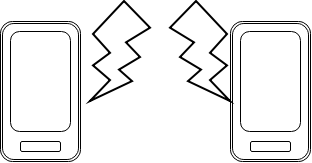
\includegraphics[clip,width=1.1\hsize]{img/beeptobeep.png}
  \caption{beeptobeep}\label{fig:beeptobeep}
\end{figure}

この手法はTPSN(time-sync Protocol for sensor network)\cite{tpsn}
などで提案されている.
原理を説明する.

端末 $A$ が自身の時刻 $t_0$ に音声パルスを発生すると,
そのパルスは音速で空間に広がり,
端末 $B$ 内の時刻 $t_1$ に受信される.
さらに,端末 $B$ からも端末 $B$ 内の時刻 $t_2$ に音声パルスを発すると,
このパルスも音速で空間に広がり,
端末 $A$ 内の時刻 $t_3$ に受信される.
ここで,図の通り,
端末 $A$ 内のパルス時間間隔 $t_3-t_0$ と
端末 $B$ 内のパルス時間間隔 $t_2-t_1$ には差が生じる(図\ref{fig:clocksynchronization}).

\begin{figure}[tb]\centering
  \hspace{-2mm}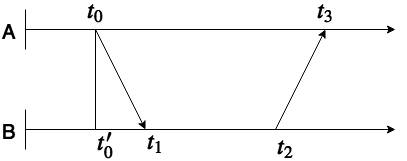
\includegraphics[clip,width=1.1\hsize]{img/clock_synchronization.png}
  \caption{clocksynchronization}\label{fig:clocksynchronization}
\end{figure}

パルスの往復で伝播にかかった時間は共に等しいと仮定すると,

$$
t_0' = t_1 - \frac{(t_3 - t_0) - (t_2 - t_1)}{2} \\
$$

となり,端末 $B$ 内時刻で端末 $A$ のパルスが発せられた時刻を推定することができる.
以上が時刻同期の原理である.

音速を $c$ とすれば,副次的に端末間の距離も求まる.

$$
d_{AB} = \frac{(t_3 - t_0) - (t_2 - t_1)}{2c}
$$

端末AB間で何らかの処理を同期的に実行したい場合は
図のようにして実行すべき時間を求められる(図\ref{fig:flowchart3}).

\begin{figure}[tb]\centering
  \hspace{-2mm}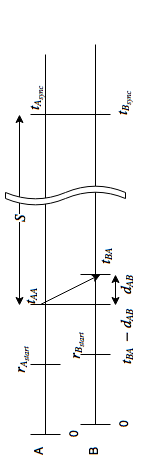
\includegraphics[clip,width=1.1\hsize]{img/flowchart3.png}
  \caption{同期実行}\label{fig:flowchart3}
\end{figure}

基準となる端末Aのパルスの受信時間およびその信号の伝達時間と,
それを受信してからの経過時間 $S$ をもとに,同期的に処理を実行できる.

こうして,端末間の時刻同期と距離測定ができた.
